\documentclass{sig-alternate}
\usepackage{subfigure}
\usepackage{graphicx}
\usepackage{url}

\clubpenalty=10000
\widowpenalty = 10000


\usepackage{amsmath,amssymb}
\usepackage{amstext}
\usepackage{dsfont}
\usepackage{xspace}
\usepackage{epsfig}
\usepackage{balance}
\usepackage[noend]{algorithmic}
\usepackage{algorithm}
\usepackage{color}
\usepackage{tikz}
\usetikzlibrary{calc}


\newtheorem{conjecture}{Conjecture}
\newtheorem{mutation}{Mutation Operator}
\newtheorem{definition}{Definition}
\newtheorem{theorem}{Theorem}
\newtheorem{lemma}{Lemma}
\newtheorem{corollary}{Corollary}
\newtheorem{claim}{Claim}

\renewcommand{\epsilon}{\varepsilon}
\newcommand{\R}{\mathds{R}}
\newcommand{\N}{\mathds{N}}
\newcommand{\Q}{\mathds{Q}}
\newcommand{\Z}{\mathds{Z}}

\begin{document}

\title{ComeTogether - an android app to meet new people}

\numberofauthors{2}
\author{
	\alignauthor Christof Ochmann\\
	\affaddr{University of Applied Sciences Zittau/G\"{o}rlitz}\\
	\affaddr{02826 G\"{o}rlitz, Germany}\\
	\email{sichochm@hs-zigr.de}\\
	\and
	\alignauthor Ingo K�rner\\
	\affaddr{University of Applied Sciences Zittau/G\"{o}rlitz}\\
	\affaddr{02826 G\"{o}rlitz, Germany}\\
	\email{siinkoer@hs-zigr.de}\\
}


\maketitle
\begin{abstract}
This work based on the document "Come-Together-App", which was created in Wirtschaftsinformatik II in a course of studies of tourism. The ideas of the project "Come-Together-App"  are realized as a prototype in "ComeTogether - an android app to meet new people". Both, frontend and backend are analysed, desgined and implemented.

\end{abstract}



\category{F.2.2}{Analysis of Algorithms and Problem Complexity}{Nonnumerical Algorithms and Problems}
\terms{Algorithms, Design, Performance, Theory}
\keywords{Parallel evolutionary algorithms, island model, spatial structures, offspring populations, runtime analysis}

\input{Ingo/Introduction}

\section{requirements engineering}\label{requirementsengineering}
Figure \ref{fig:useCaseDiagram} shows the use case diagram for ComeTogether.

\section{Design}\label{Design}

In figure \ref{fig:UserServiceREST} you can see the design for the UserService. UserServiceREST encapsulate the REST-Functionality of the UserService. UserPersistence access database with prepared statements p.e. to save, read or delete users. Between UserServiceREST and UserPersistence are service class and DAO class to encapsulate different levels of abstraction. Beside UserServiceREST there are the classes EventServiceREST, ParticipationServiceREST and MessageServiceREST. EventServiceREST in figure \ref{fig:EventServiceREST} creates, reads and deletes events. ParticipationServiceREST in figure \ref{fig:ParticipationServiceREST} creates participations and gives back a list of participation for a given eventid or a given userid. MessageServiceREST in figure \ref{fig:MessageServiceREST} creates, reads or deletes messages.

\begin{figure}[htp]
\centering
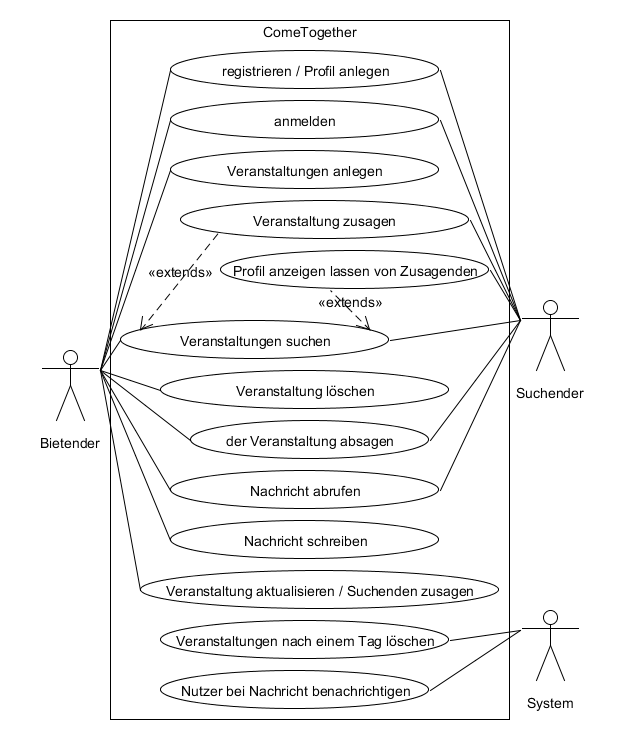
\includegraphics[width=0.5\textwidth]{Ingo/pictures/UseCaseDiagram.png}
\caption{use case diagram}
\label{fig:useCaseDiagram}
\end{figure}


\begin{figure}[htp]
\centering
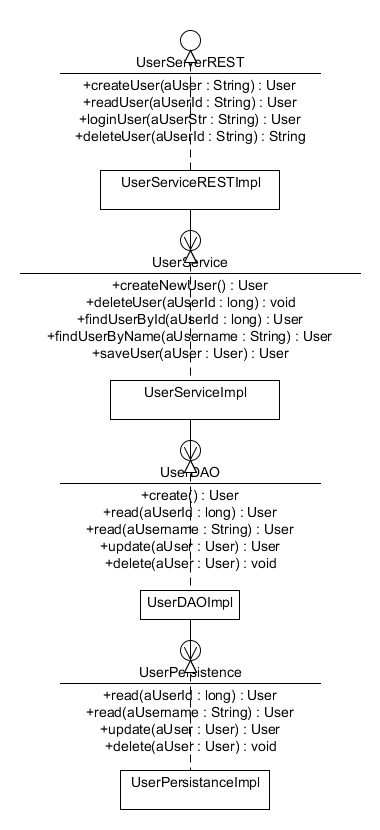
\includegraphics[width=0.5\textwidth]{Ingo/pictures/Design_User.png}
\caption{desing class diagramm UserServiceREST}
\label{fig:UserServiceREST}
\end{figure}


\begin{figure}[htp]
\centering
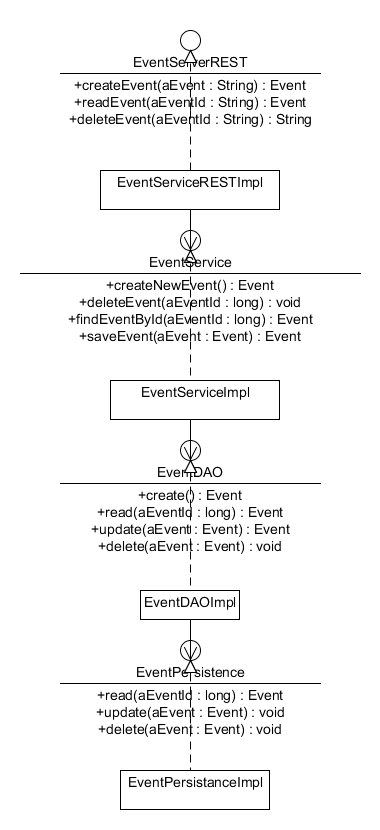
\includegraphics[width=0.5\textwidth]{Ingo/pictures/Design_Event.png}
\caption{desing class diagramm EventServiceREST}
\label{fig:EventServiceREST}
\end{figure}


\begin{figure}[htp]
\centering
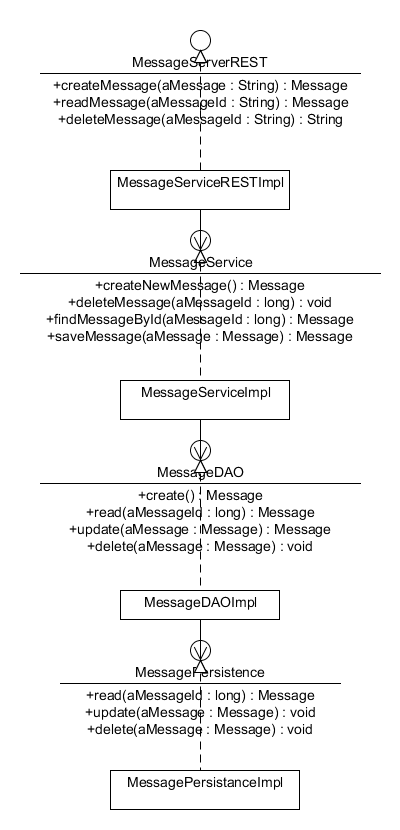
\includegraphics[width=0.5\textwidth]{Ingo/pictures/Design_Message.png}
\caption{desing class diagramm MessageServiceREST}
\label{fig:MessageServiceREST}
\end{figure}


\begin{figure}[htp]
\centering
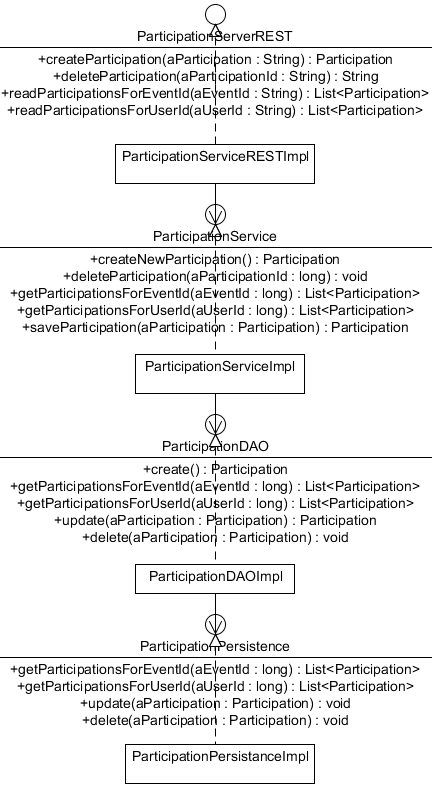
\includegraphics[width=0.5\textwidth]{Ingo/pictures/Design_Participation.png}
\caption{desing class diagramm ParticipationServiceREST}
\label{fig:ParticipationServiceREST}
\end{figure}

\section{database}\label{database}
In figure \ref{fig:EERdiagram} you can see the data base design of ComeTogether.

\begin{figure}[htp]
\centering
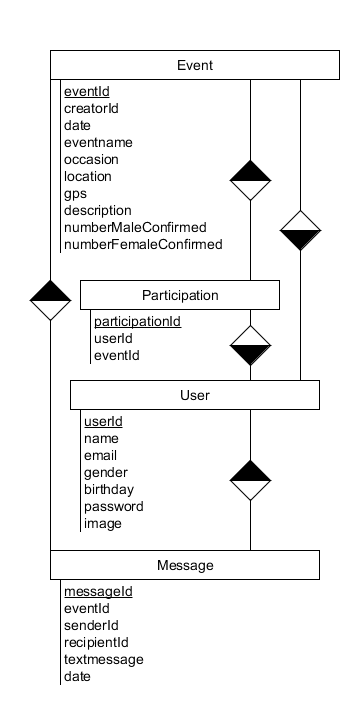
\includegraphics[width=0.5\textwidth]{Ingo/pictures/EER-diagram.png}
\caption{eer-diagram}
\label{fig:EERdiagram}
\end{figure}

Parallelization is becoming a more and more important issue for solving difficult optimization problems~\cite{Alba2005}. Evolutionary Algorithms (EAs) are known to be one of the most successful strategies to find good solutions of hard optimization problems for which no efficient methods are known. For large-scale applications it is common to use parallel implementations, which have shown to be a successful strategy to speed up the computation in many cases \cite{Alba2002,Tomassini2005}.
Especially due to current multi-core architectures, parallel evolutionary algorithms are highly relevant \cite{Cant'u-Paz1999,Tomassini2005}.

A simple way of using parallelization is to use offspring populations, where offspring are created and evaluated on different processors. Island models use parallelization on a higher level. Subpopulations, called islands, evolve independently for some time and periodically exchange individuals in a process called migration. Islands are usually spatially structured, with communication taking place on a communication topology connecting the islands.
Despite many wide-spread applications and a long history of such parallel EAs, the theory of these algorithms is not well developed and more fundamental research is needed~\cite{Skolicki2005}.

The most obvious goal of parallelization is to obtain a good speedup, defined as the quotient of the total optimization time such as the total number of function evaluations in an EA and the parallel optimization time such as the number of generations.
(Asymptotic) linear speedups are achieved when the parallel running time is (asymptotically) the total optimization time divided by the number of processors.
Recently, L�ssig and Sudholt~\cite{Lassig2010,Lassig2010b} presented a constructed function where an exponential speedup could be shown.
In~\cite{Lassig2010a} they provided general methods for analyzing expected parallel optimization times---and hence speedups---by adapting the well-known fitness level method. This was applied to island models with different migration topologies~\cite{Lassig2010a} such as ring graphs, torus graphs, and complete graphs for basic test functions such as ....

An open question is how island models perform in more practical settings such as combinatorial optimization where many analyses of (non-parallel) EAs have been obtained~\cite{BookNeuWit}. Therefore, we present such an analysis, considering speedups by parallelization for different combinatorial problems: sorting as an optimization problem~\cite{Scharnow2004} (Section~\ref{sec:Sorting}), the single-source shortest path problem~\cite{doerr2008tight,Doerr2010} (Section~\ref{sec:ShortestPaths}), and the Eulerian cycle problem with different genotype representations and operators~\cite{Doerr2007,Doerr2007a,neumann2008expected} (Section~\ref{sec:EulerianCycles}).

The goal is to investigate the possible speedups, identify settings where parallelization is most useful, and give answers to many design questions that come with island models such as how to choose the number of islands or the frequency of migration.
Although these problems are easy from the perspective of computational complexity, our investigations give insight into how parallel EAs deal with characteristics of different problem classes, such as plateaus of equal fitness. This leads to interesting insights and paves the way for further investigations, including NP-hard problems.

\section{Preliminaries}
\label{sec:Preliminaries}

The idea of an island model is to have separate subpopulations evolving independently for some time. ....


\section{Previous Work}
\label{sec:PreviousWork}

L{\"a}ssig and Sudholt~\cite{Lassig2010a,Lassig2011} presented general bounds for parallel EAs using the \emph{fitness-level method} or \emph{method of $f$-based partitions}. The idea is to divide the search space into sets $A_1, \dots, A_m$ strictly ordered w.\,r.\,t.\ fitness: $A_1 <_f A_2 <_f \dots <_f A_m$ where $A <_f B$ iff $f(a) < f(b)$ for every $a \in A, b \in B$. In addition, $A_m$ contains only global optima.

We say that a population-based search algorithm (this includes populations of size 1) is in $A_i$ or on level~$i$ if the current best individual in the population is in $A_i$. Elitist algorithms (i.\,e. algorithms where the best solution in the population never worsens) can only increase the current level. The goal of the optimization is to reach~$A_m$.

In the worst case an algorithm has to traverse all fitness levels $A_i, A_{i+1}, \dots, A_m$ if it starts in $A_i$. Now, if $s_i$ is a lower bound on the probability of leaving $A_i$ towards any higher fitness level in one generation, the expected time until this happens is at most the reciprocal, $1/s_i$. We then get that the optimization time is bounded by $\sum_{i=1}^{m-1} 1/s_i$.

The fitness-level method gives good bounds in case a search algorithm typically does not skip too many fitness levels and the probabilities of finding improvements from any set $A_i$ are similar for all search points in $A_i$. It only yields crude upper bounds in case there are difficult fitness levels that are skipped with a very high probability.

The perspective used when arguing with fitness levels is very well suited for parallelization. The search for improvements is given by Bernoulli trials: in every generation there is a chance of finding an improvement.
While waiting for improvements to be found, parallelizing these trials on different processors easily leads to good speedups.
L{\"a}ssig and Sudholt~\cite{Lassig2010a} have made this precise for island models that run elitist islands. If migration is used in every generation, information about the current best fitness level is propagated to neighbored islands. This increases the number of islands on the current best fitness level and thus the number of processors that search for better fitness levels in parallel.

The following theorem summarizes their results. The bounds for rings and torus graphs are refined towards bounds that hold for arbitrary numbers of islands; the theorems in~\cite{Lassig2010a} were restricted to large enough numbers. Our refined theorem allows for better insight into which numbers of islands lead to a linear speedup (asymptotically).
A directed graph is strongly connected if for every two vertices $u, v$ there is a directed path from~$u$ to~$v$ and vice versa.
\begin{theorem}
\label{the:generalBounds}
Consider an island model with $\mu$ islands ...
\end{theorem}
\begin{proof}
The third claim is a special case of Theorem~8 in~\cite{Lassig2010a} (results in~\cite{Lassig2010a} also accounted for stochastic migrations), allowing for a better constant in the factor $2/\mu$.

The first bound is a refinement of Theorem~3 in~\cite{Lassig2010a}. In the proof of this theorem it is shown that for every integer $k \le \mu$ the expected time until fitness level~$i$ is left is bounded by $k + \frac{2}{k} \cdot \frac{1}{s_i}$.
Now, if $\mu \ge k := s_i^{-1/2}$ (ignoring rounding issues), the expected number of generations on fitness level~$i$ is bounded by $k + 2/k \cdot s_i^{-1} = s^{-1/2} + 2s^{-1/2}$. If $\mu < s_i^{-1/2}$, we get for $k := \mu$ an upper bound of $\mu + 2/\mu \cdot s_i^{-1} > s_i^{-1/2} + 2/\mu \cdot s_i^{-1}$. Together, this proves the claimed bound.

Likewise, the second bound refines Theorem~4 in~\cite{Lassig2010a} where it was proven that the expected time for leaving level~$i$ is at most $8\sqrt{k} + \frac{2}{k} \cdot \frac{1}{s_i}$. If $\mu \ge k := s_i^{-2/3}$, this gives $8s_i^{-1/3} + 2 s_i^{-1/3} = 10 s_i^{-1/3}$. Otherwise, $k := \mu$ yields a bound of $8\sqrt{\mu} + \frac{2}{\mu} \cdot \frac{1}{s_i} \le 8s_i^{-1/3} + \frac{2}{\mu} \cdot \frac{1}{s_i}$.
\end{proof}

Assuming the fitness-level bound for the time $\sum_{i=1}^{m-1} \frac{1}{s_i}$ of a single island is asymptotically tight, all three bounds yield an asymptotic linear speedup in case the first summands are each of at most the same order as the second summand.

Besides the mentioned works, parallel models, including offspring populations, have also been considered in other theoretical studies of EAs in combinatorial optimization.
...

\section{Sorting}
\label{sec:Sorting}

...


\section{Shortest Paths}
\label{sec:ShortestPaths}


...


\section{Eulerian Cycles}
\label{sec:EulerianCycles}

...

\subsection{Edge Walks}

...

\subsection{Restricted Mutation Operators}

...

\subsection{Adjacency List Matchings}

...

\section{Conclusions}
\label{sec:Conclusions}

Considering speedups of island models has led to a surprising richness of results. For sorting linear speedups are possible, but only for $\mu = O(\log n)$ islands. The single-source shortest paths problem allows for linear speedups, the maximum number of islands depending on the topology and the mutation operator. For $K_\mu$ or offspring populations almost quadratic factors can be gained. For Eulerian cycles and the edge walk representation speedups on the instance $G'$ vary grossly from exponential up to $\mu = O(\log m)$ for rare or no migrations to at most logarithmic speedups, if migration is used too frequently. This is due to the existence of plateaus of equal fitness. Again, results vary with the mutation operator and the representation. The most efficient representation, adjacency list matchings, turned out to be parallelizable efficiently in a straightforward way.

\subsection*{Acknowledgments}
The authors would like to thank .....the German fast food industry for keeping us alive.

\bibliographystyle{abbrv}
\bibliography{literature-short}
\balance

\end{document}
